\section{Définitions : }
\begin{center}
	\color[rgb]{0.2, 0.6, 0.2} Mais alors qu'est-ce que le Big Data ?
\end{center}

Plusieurs définitions peuvent être données au Big Data, étant un objet complexe polymorphe, sa définition varie. Parmi elles nous citons :

\begin{description}

	\item[Définition 1:]Le Big Data désigne l'ensemble des données numériques produites par l'utilisation des nouvelles technologies à des fins personnelles ou professionnelles. Cela regroupe les données d'entreprise ? Des contenus publiés sur le web, des transactions de commerce électronique, des échanges sur les réseaux sociaux, des données transmises par les objets connectés des données géolocalisées, ...etc. \cite{Def1}
	
	\item[Définition 2:]Le "Big Data" désigne les technologies et les initiatives qui impliquent des données trop diverses, en évolution rapide ou massives pour que les technologies, les compétences et les infrastructures conventionnelles puissent être traitées efficacement. Autrement dit, le volume, la vitesse ou la variété des données est trop important. \cite{Def2}
	
	\item[Définition 3:]Le terme Big Data fait référence aux données dont le coût de stockage, de gestion et d'analyse dans des systèmes de base de données traditionnels (relationnels et/ou monolithiques) serait généralement trop élevé. Habituellement, ces systèmes ne sont pas rentables, car ils ne disposent pas de la flexibilité nécessaire pour stocker des données non structurées (comme des images, du texte et des vidéos), pour accommoder des données "à haute vélocité" (en temps réel) ou pour s'adapter automatiquement à de très gros volumes de données (de l'ordre du pétaoctet). \cite{Def3}
	
\end{description}

\begin{figure}[h]
	\centering
	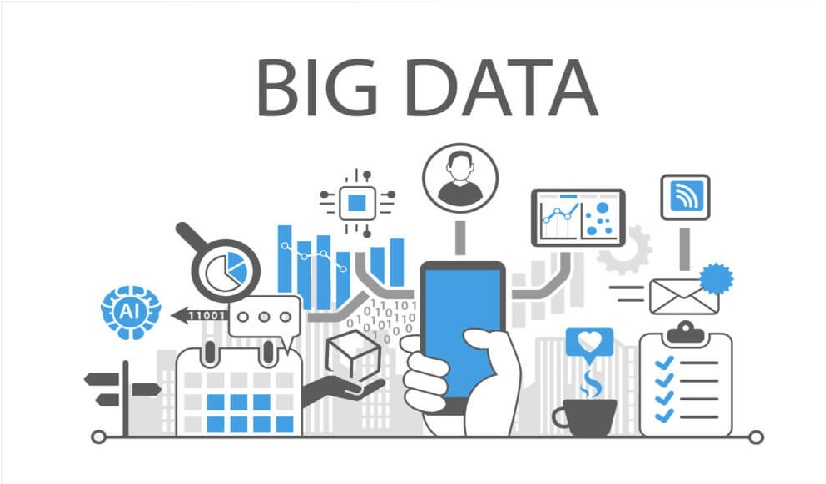
\includegraphics[scale=0.6]{img/part1/1.2}
	\caption{Le Big Data}
\end{figure}